% Options for packages loaded elsewhere
\PassOptionsToPackage{unicode}{hyperref}
\PassOptionsToPackage{hyphens}{url}
%
\documentclass[
  12pt,
]{article}
\usepackage{amsmath,amssymb}
\usepackage{iftex}
\ifPDFTeX
  \usepackage[T1]{fontenc}
  \usepackage[utf8]{inputenc}
  \usepackage{textcomp} % provide euro and other symbols
\else % if luatex or xetex
  \usepackage{unicode-math} % this also loads fontspec
  \defaultfontfeatures{Scale=MatchLowercase}
  \defaultfontfeatures[\rmfamily]{Ligatures=TeX,Scale=1}
\fi
\usepackage{lmodern}
\ifPDFTeX\else
  % xetex/luatex font selection
\fi
% Use upquote if available, for straight quotes in verbatim environments
\IfFileExists{upquote.sty}{\usepackage{upquote}}{}
\IfFileExists{microtype.sty}{% use microtype if available
  \usepackage[]{microtype}
  \UseMicrotypeSet[protrusion]{basicmath} % disable protrusion for tt fonts
}{}
\makeatletter
\@ifundefined{KOMAClassName}{% if non-KOMA class
  \IfFileExists{parskip.sty}{%
    \usepackage{parskip}
  }{% else
    \setlength{\parindent}{0pt}
    \setlength{\parskip}{6pt plus 2pt minus 1pt}}
}{% if KOMA class
  \KOMAoptions{parskip=half}}
\makeatother
\usepackage{xcolor}
\usepackage[margin=1in]{geometry}
\usepackage{longtable,booktabs,array}
\usepackage{calc} % for calculating minipage widths
% Correct order of tables after \paragraph or \subparagraph
\usepackage{etoolbox}
\makeatletter
\patchcmd\longtable{\par}{\if@noskipsec\mbox{}\fi\par}{}{}
\makeatother
% Allow footnotes in longtable head/foot
\IfFileExists{footnotehyper.sty}{\usepackage{footnotehyper}}{\usepackage{footnote}}
\makesavenoteenv{longtable}
\usepackage{graphicx}
\makeatletter
\def\maxwidth{\ifdim\Gin@nat@width>\linewidth\linewidth\else\Gin@nat@width\fi}
\def\maxheight{\ifdim\Gin@nat@height>\textheight\textheight\else\Gin@nat@height\fi}
\makeatother
% Scale images if necessary, so that they will not overflow the page
% margins by default, and it is still possible to overwrite the defaults
% using explicit options in \includegraphics[width, height, ...]{}
\setkeys{Gin}{width=\maxwidth,height=\maxheight,keepaspectratio}
% Set default figure placement to htbp
\makeatletter
\def\fps@figure{htbp}
\makeatother
\setlength{\emergencystretch}{3em} % prevent overfull lines
\providecommand{\tightlist}{%
  \setlength{\itemsep}{0pt}\setlength{\parskip}{0pt}}
\setcounter{secnumdepth}{5}
\usepackage[OT4]{polski}
\usepackage[utf8]{inputenc}
\usepackage{graphicx}
\usepackage{float}
\usepackage{xcolor}
\usepackage{booktabs}
\usepackage{longtable}
\usepackage{array}
\usepackage{multirow}
\usepackage{wrapfig}
\usepackage{float}
\usepackage{colortbl}
\usepackage{pdflscape}
\usepackage{tabu}
\usepackage{threeparttable}
\usepackage{threeparttablex}
\usepackage[normalem]{ulem}
\usepackage{makecell}
\usepackage{xcolor}
\ifLuaTeX
  \usepackage{selnolig}  % disable illegal ligatures
\fi
\usepackage{bookmark}
\IfFileExists{xurl.sty}{\usepackage{xurl}}{} % add URL line breaks if available
\urlstyle{same}
\hypersetup{
  pdftitle={Sprawozdanie 2},
  pdfauthor={Kacper Szmigielski, 282255 i Mateusz Wizner, 277508},
  hidelinks,
  pdfcreator={LaTeX via pandoc}}

\title{Sprawozdanie 2}
\usepackage{etoolbox}
\makeatletter
\providecommand{\subtitle}[1]{% add subtitle to \maketitle
  \apptocmd{\@title}{\par {\large #1 \par}}{}{}
}
\makeatother
\subtitle{Eksploracja danych}
\author{Kacper Szmigielski, 282255 i Mateusz Wizner, 277508}
\date{2025-04-29}

\begin{document}
\maketitle

{
\setcounter{tocdepth}{3}
\tableofcontents
}
\section{ZADANIE 1 (Dyskretyzacja(przedziałowanie) cech
ciągłych)}\label{zadanie-1-dyskretyzacjaprzedziaux142owanie-cech-ciux105gux142ych}

\subsection{a) Dane: iris (R-pakiet
datasets).}\label{a-dane-iris-r-pakiet-datasets.}

\textbf{3} Pierwsze wiersze z pakietu iris

Zbiór danych zawiera wyniki pomiarów uzyskanych dla \textbf{trzech
gatunków irysów} (tj. setosa, versicolor i virginica) i został
\textbf{udostępniony przez Ronalda Fishera w roku 1936.}

-- \textbf{Pomiary} dotyczą \textbf{długości oraz szerokości} dwóch
różnych części kwiatu-- działki \textbf{kielicha (ang. sepal) oraz
płatka (ang. petal).}

\subsection{b) Wybór cech}\label{b-wybuxf3r-cech}

\textbf{Szukamy cech, których róznice są najbardziej spójne z różnicami
pomiędzy gatunkami.}

\begin{center}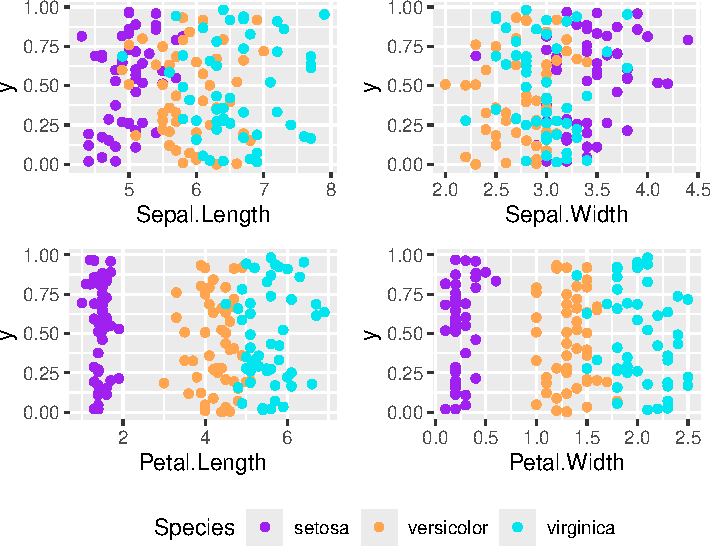
\includegraphics{Sprawozdanie2_files/figure-latex/zad1b1-1} \end{center}

Po przeanalizowaniu scatter-plotów, widać ,że podczas szukania cechy o
najlepszej zdolności dyskryminacyjnej warto zwrócić uwagę na
\textbf{Petal.Length i Petal.Width}, natomiast jeżeli poszukujemy
kolumny o najgorszej zdolności dyskryminacyjnej to wybór rozsztrzygamy
spośród \textbf{Sepal.Length i Sepal.Width}

Musimy jednak wybrać \textbf{wartości najlepsze i najgorsze} do
dyksryminacji, aby to zrobić przeanalizujemy \textbf{box-ploty}.

\begin{center}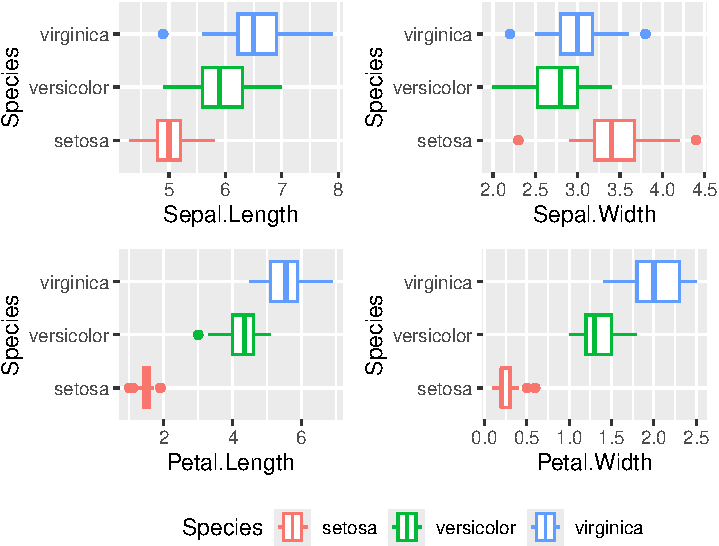
\includegraphics{Sprawozdanie2_files/figure-latex/zad1b2-1} \end{center}

Na ich podstawie możemy uznać, że \textbf{Petal.Width może stanowić
najlepszy wyznacznik gatunku} roślin \textbf{Najgorszym natomiast jest}
\textbf{Sepal.Width}. Ponieważ dla \textbf{Petal.Width} gatunki w
najmniejszym stopniu się pokrywają ze względu na tą cechę , a w
\textbf{Sepal.Width} w największym.

\subsection{c) Porównanie nienadzorowanych metod
dyskretyzacji}\label{c-poruxf3wnanie-nienadzorowanych-metod-dyskretyzacji}

\subsubsection{Metoda : Równe
częstości(Frequency)}\label{metoda-ruxf3wne-czux119stoux15bcifrequency}

\paragraph{Dla najlepszej cechy : Petal.Length
(Frequency)}\label{dla-najlepszej-cechy-petal.length-frequency}

\begin{center}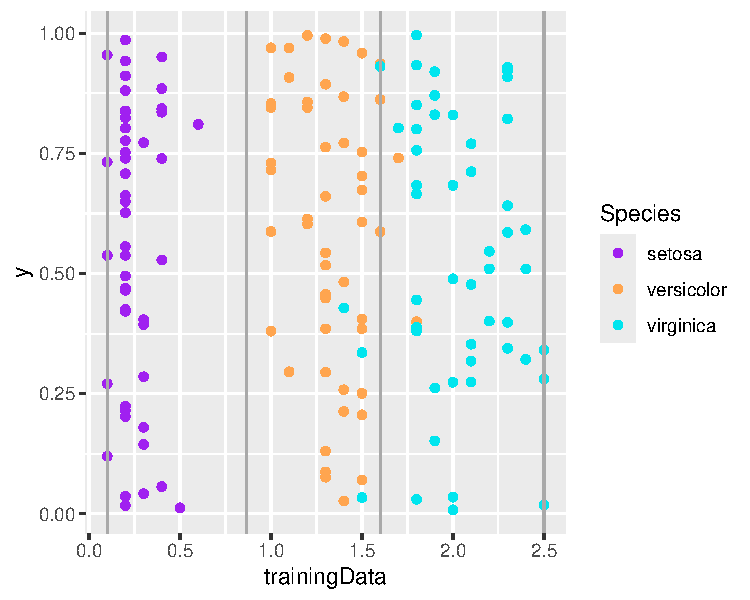
\includegraphics{Sprawozdanie2_files/figure-latex/frequences_najl-1} \end{center}

Widać, że linie uzyskane za pomocną \textbf{Frequency} dość do dobrze
rozdzielają nasze dane .

Jeżeli chcemy dokłądniej przeanalizować zależność podziału od gatunków,
narysujemy specjalne bar-ploty

\begin{center}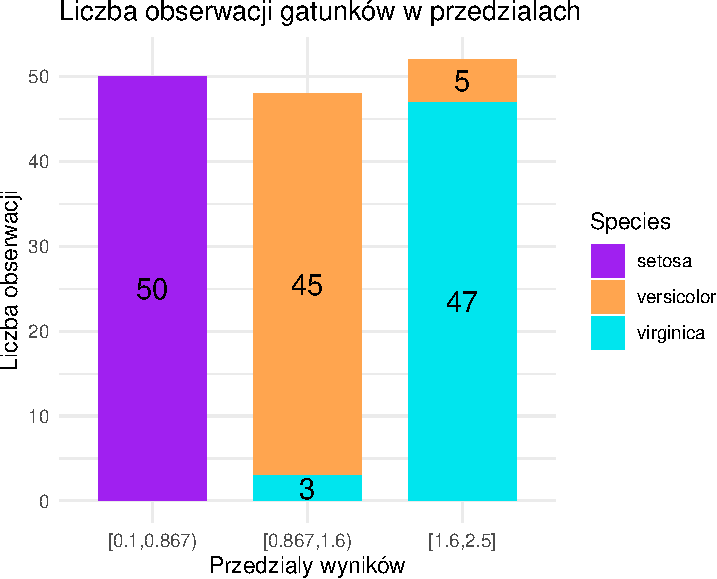
\includegraphics{Sprawozdanie2_files/figure-latex/tabela_kondygnacji_1_najl-1} \end{center}

Świadczą one o tym ,że metoda Frequency dla zmiennej Petal.Width
bezproblemowo oddziela gatunek setosa, lecz wśród pozostałych występuje
zjawisko mieszania się (3 virginica przyporządkowano do versicolor, a 5
versicolor do virginica)

W przypadku tej metody \textbf{zgodność} uzyskanego grupowania z
realnymi wartościami \textbf{wynosi} :

\begin{verbatim}
## [1] 0.9466667
\end{verbatim}

\paragraph{Dla najgorszej cechy : Sepal.Length
(Frequency)}\label{dla-najgorszej-cechy-sepal.length-frequency}

\begin{center}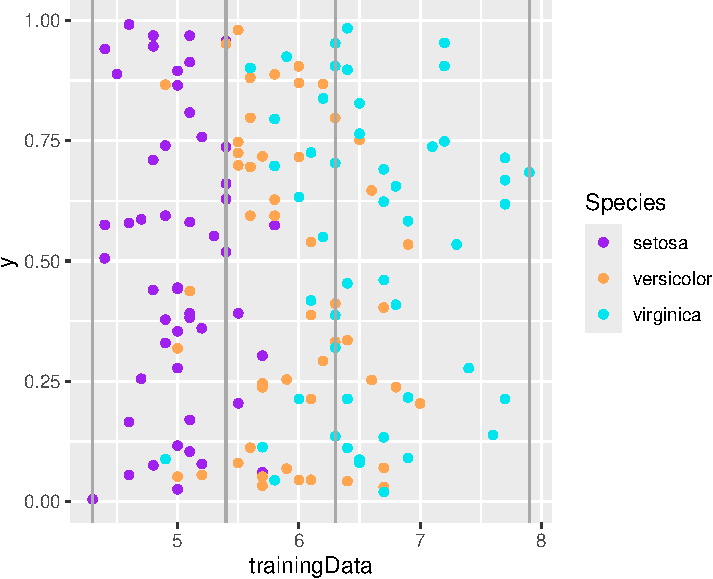
\includegraphics{Sprawozdanie2_files/figure-latex/frequences_najg-1} \end{center}

Scatter-plot wskazuje, że dla Sepal.Length grupowanie może być dość
problematyczne, widać, że obserwacje są dość wymieszane, i trudno będzie
w prosty sposób oddzielić je tak, aby gatunki były prawidłowo
rozłożożone, te sam problem pojawia się w pozostałych metodach grupowań,
dlatego scatter-plot Sepal.Length analizujemy tylko tutaj.

\begin{center}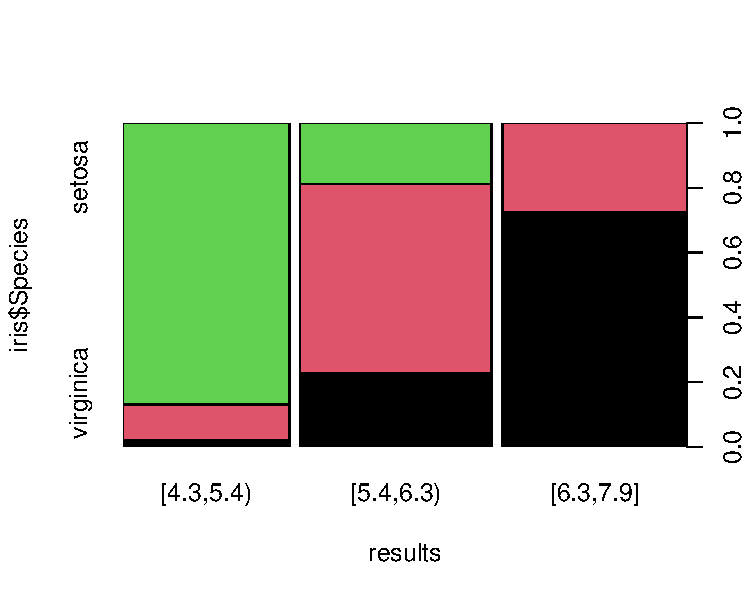
\includegraphics{Sprawozdanie2_files/figure-latex/tabela_kondygnacji_1_najg-1} \end{center}

Na tabeli przyporządkowań widać, problemy metody Frequency, przy
grupowaniu dla zmiennej Sepal.Length, gatunki są dość mocno
przemieszane, brakuje jednolitego podziału.

\begin{verbatim}
## [1] 0.72
\end{verbatim}

Zgodność dla nagjroszej cechy wynosi jedynie ok \textbf{72\%}, co mówi o
znacznym spadku wiarygodności (\textbf{o ok 23 \%}) w porównaniu do
Petal.Width

\subsubsection{Metoda : Równe szerokości
(Interval)}\label{metoda-ruxf3wne-szerokoux15bci-interval}

\paragraph{Dla najlepszej cechy : Petal.Width
(Interval)}\label{dla-najlepszej-cechy-petal.width-interval}

\begin{center}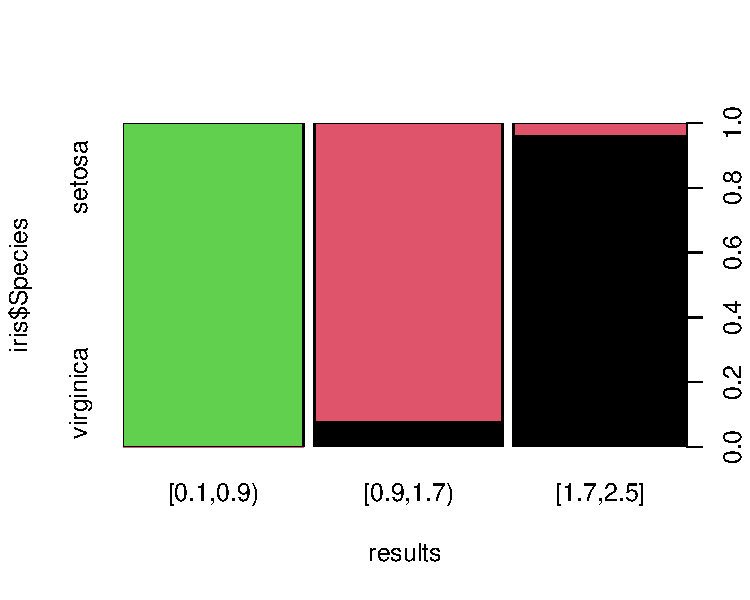
\includegraphics{Sprawozdanie2_files/figure-latex/tabela_kondygnacji_2_najl-1} \end{center}

Po tabeli przyporządkowań widać, że mamy trocjhę lepsze odróżnienienie
versicolor od virginica

Dla tej metody również mamy \textbf{zgodność na poziomie} :

\begin{verbatim}
## [1] 0.96
\end{verbatim}

Widać lekki wzrost zgodności w porównaniu do poprzedniej metody
(\textbf{o ok 1\%})

\paragraph{Dla najgorszej cechy ; Sepal.Length
(Interval)}\label{dla-najgorszej-cechy-sepal.length-interval}

\begin{center}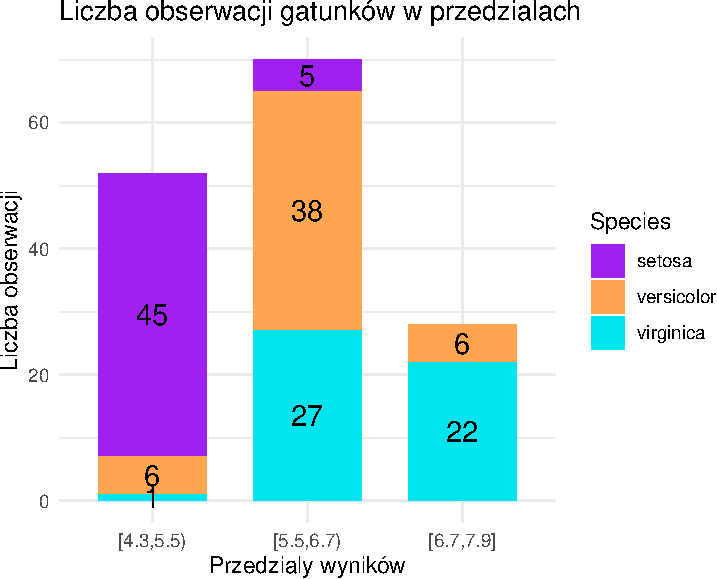
\includegraphics{Sprawozdanie2_files/figure-latex/tabela_kondygnacji_2_najg-1} \end{center}

Dla tabeli zgodności widać, że metoda w zły sposób rozdziela przypadki,
bardzo duża ich ilość znajduje się w środkowym przedziale, nie jest to
dobry podział gatunkowy

Metoda ta, dla najgorszzej cechy dyksryminuje ze zgodnością :

\begin{verbatim}
## [1] 0.5729167
\end{verbatim}

Czyli w porównaniu do metody Frequency mamy \textbf{spadek} aż \textbf{o
ok 16\%}

\subsubsection{Metoda : k najbliższych sąsiadów
(K-means)}\label{metoda-k-najbliux17cszych-sux105siaduxf3w-k-means}

\paragraph{Dla najlepszej cechy : Petal.Width
(K-means)}\label{dla-najlepszej-cechy-petal.width-k-means}

\begin{center}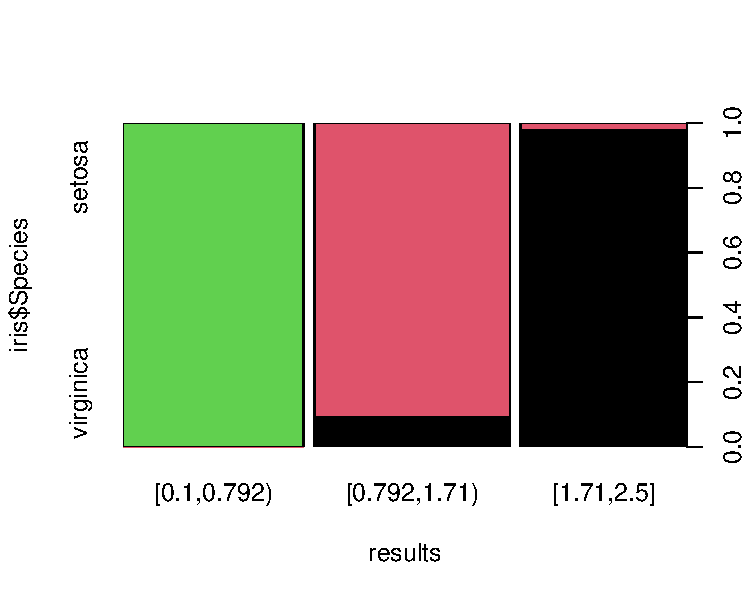
\includegraphics{Sprawozdanie2_files/figure-latex/tabela_kondygnacji_3_najl-1} \end{center}

Analogiczny podział jak w poprzedniej metodzie

Zgodność na poziomie :

\begin{verbatim}
## [1] 0.96
\end{verbatim}

Lepsza \textbf{o ok 3\%} od ubiegłej metody

\paragraph{Dla najgorszej cechy : Sepal.Length
(K-means)}\label{dla-najgorszej-cechy-sepal.length-k-means}

\begin{center}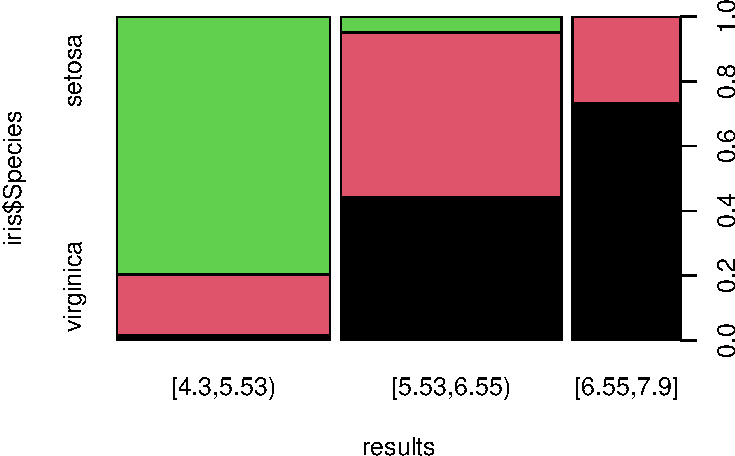
\includegraphics{Sprawozdanie2_files/figure-latex/tabela_kondygnacji_3_najg-1} \end{center}

Bardziej równomierne rozłożenie jak w metodzie ubiegłej, lecz nie jest
wciąż nie jest dobre pod względem gatunkowym

Dla najgorszej cechy mamy zgodność :

\begin{verbatim}
## [1] 0.7266667
\end{verbatim}

W tym przypadku jest ona \textbf{na poziome metody Frequency (gorsza o
1)}

\subsubsection{Dyskretyzacja z przedziałami zadanymi przez urzytkownika
(fixed)}\label{dyskretyzacja-z-przedziaux142ami-zadanymi-przez-urzytkownika-fixed}

\paragraph{Dla najlepszej cechy : Petal.Width
(fixed)}\label{dla-najlepszej-cechy-petal.width-fixed}

\begin{center}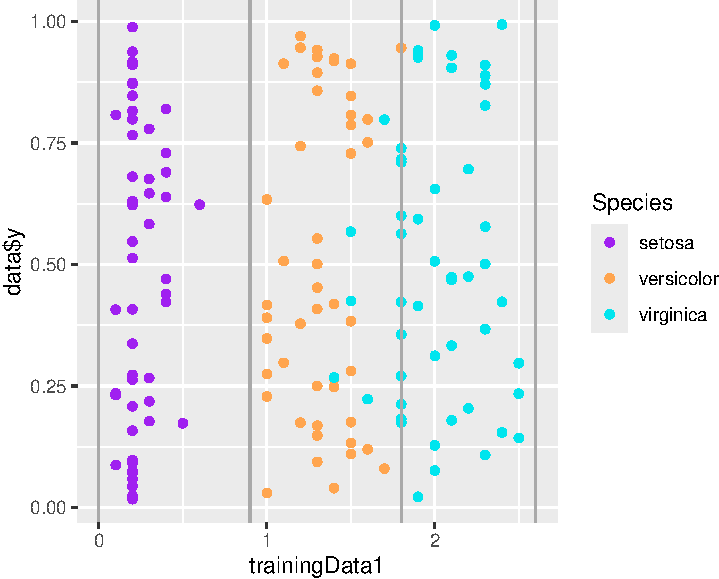
\includegraphics{Sprawozdanie2_files/figure-latex/givenRanges_najl-1} \end{center}

Na wykresie mamy zaznaczone też końce przedziałów, to jest potrzebne, co
jest potrzebne podczas rysowania kolejnego wykresu

\begin{center}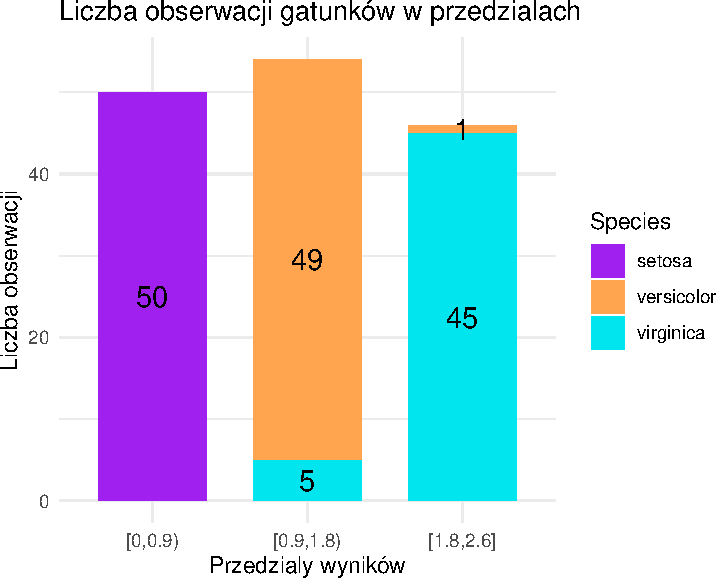
\includegraphics{Sprawozdanie2_files/figure-latex/tabela_kondygnacji_4_najl-1} \end{center}

Mamy najmniejsze rozmieszanie virignica i versicolor,tylko jedna
versicolor została, źle przyporządkowana, ale aż 5 virginic zostało źle
rozgrupowanych

Zgodność na poziome poprzednich dwóch metod, wynosi :

\begin{verbatim}
## [1] 0.96
\end{verbatim}

\paragraph{Dla najgorszej cechy : Sepal.Length
(fixed)}\label{dla-najgorszej-cechy-sepal.length-fixed}

\begin{center}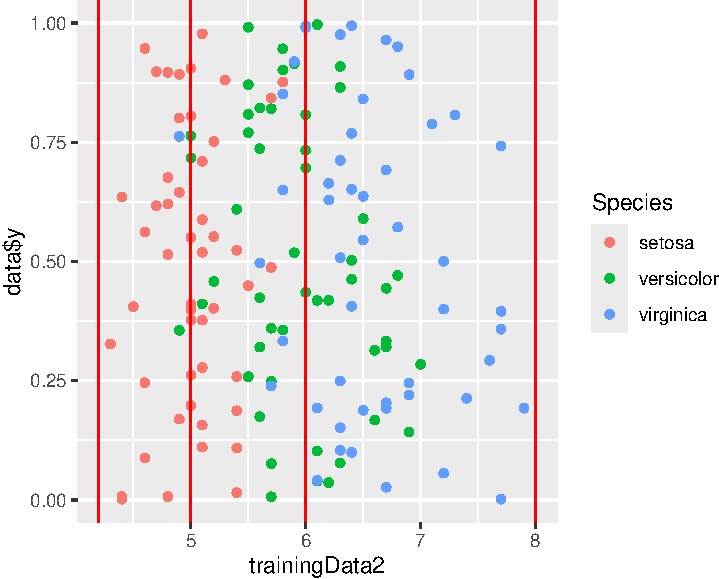
\includegraphics{Sprawozdanie2_files/figure-latex/givenRanges_najg-1} \end{center}

\begin{center}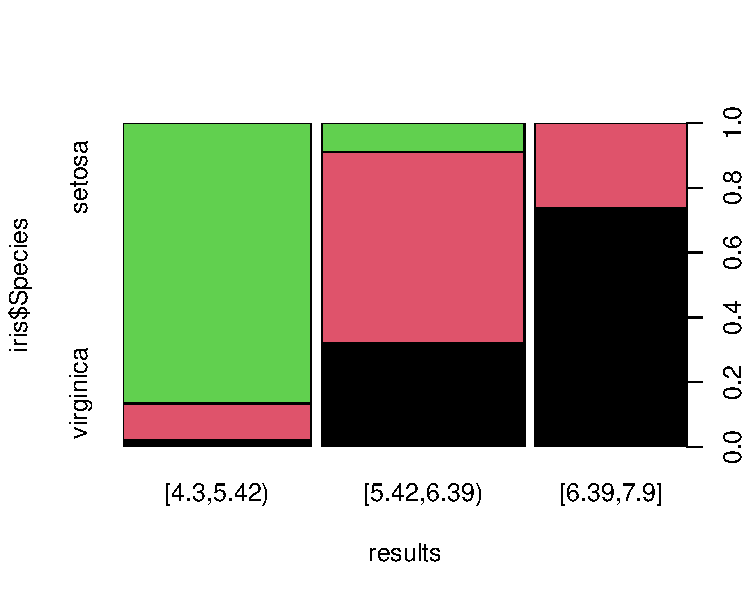
\includegraphics{Sprawozdanie2_files/figure-latex/tabela_kondygnacji_4_najg-1} \end{center}

Znaczącą przewaga obserwacji w środkowym przedziale

Dla cechy o najgorszej zdolności dyskryminacyjnej :

\begin{verbatim}
## [1] 0.72
\end{verbatim}

\subsection{Wnioski :}\label{wnioski}

\textbf{Porównamy teraz} zgodności procentowe \textbf{wyników}, dla
\textbf{poszczególnych algorytmów}

\begin{longtable}[]{@{}lrrrr@{}}
\toprule\noalign{}
& frequency & interval & cluster & fixed \\
\midrule\noalign{}
\endhead
\bottomrule\noalign{}
\endlastfoot
Petal.Width & 0.9466667 & 0.9600000 & 0.9600000 & 0.96 \\
Sepal.Length & 0.7200000 & 0.5729167 & 0.7266667 & 0.72 \\
\end{longtable}

Na podstawie tabeli, dokłądniej \textbf{Porównania przyporządkować dla
cech najgorszych i najlepszych pod względem dyskryminacji}. Możemy
wnioskować, że dla obecnych danych \textbf{najlepszym algorytmem}
\textbf{jest frequency(częstość)} odznacza się najlepszym
przyporządkowaniem zarówno dla Sepal.Length jak i Petal.Width

\section{ZADANIE 2 (Analizaskładowych głównych (Principal Component
Analysis
(PCA)))}\label{zadanie-2-analizaskux142adowych-gux142uxf3wnych-principal-component-analysis-pca}

\subsection{a) Przygotowanie danych}\label{a-przygotowanie-danych}

\begin{longtable}[]{@{}lr@{}}
\caption{Podstawowe informacje nt. danych
\texttt{uaScoresDataFrame}}\tabularnewline
\toprule\noalign{}
\endfirsthead
\endhead
\bottomrule\noalign{}
\endlastfoot
rows & 266 \\
columns & 21 \\
discrete\_columns & 3 \\
continuous\_columns & 18 \\
all\_missing\_columns & 0 \\
total\_missing\_values & 0 \\
complete\_rows & 266 \\
total\_observations & 5586 \\
memory\_usage & 73496 \\
\end{longtable}

Typy danych w zbiorze

\begin{center}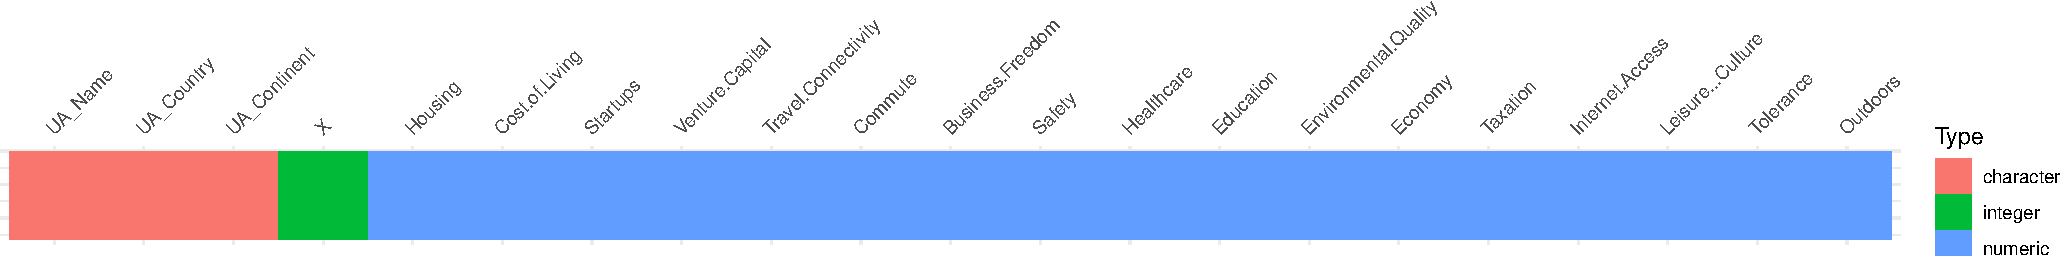
\includegraphics{Sprawozdanie2_files/figure-latex/typy_danych-1} \end{center}

\begin{center}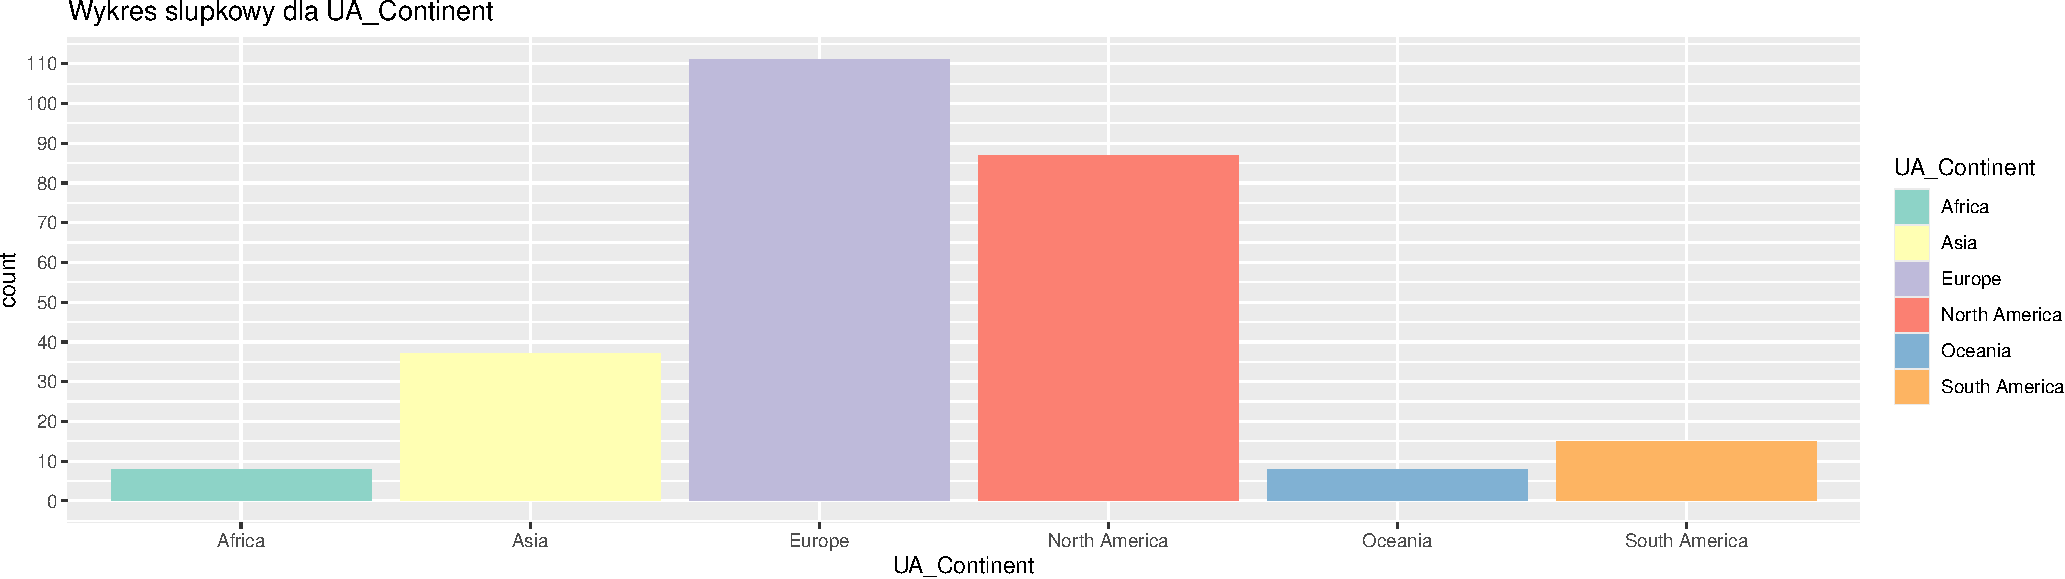
\includegraphics{Sprawozdanie2_files/figure-latex/wykresy_jakosciowe-1} \end{center}

\begin{center}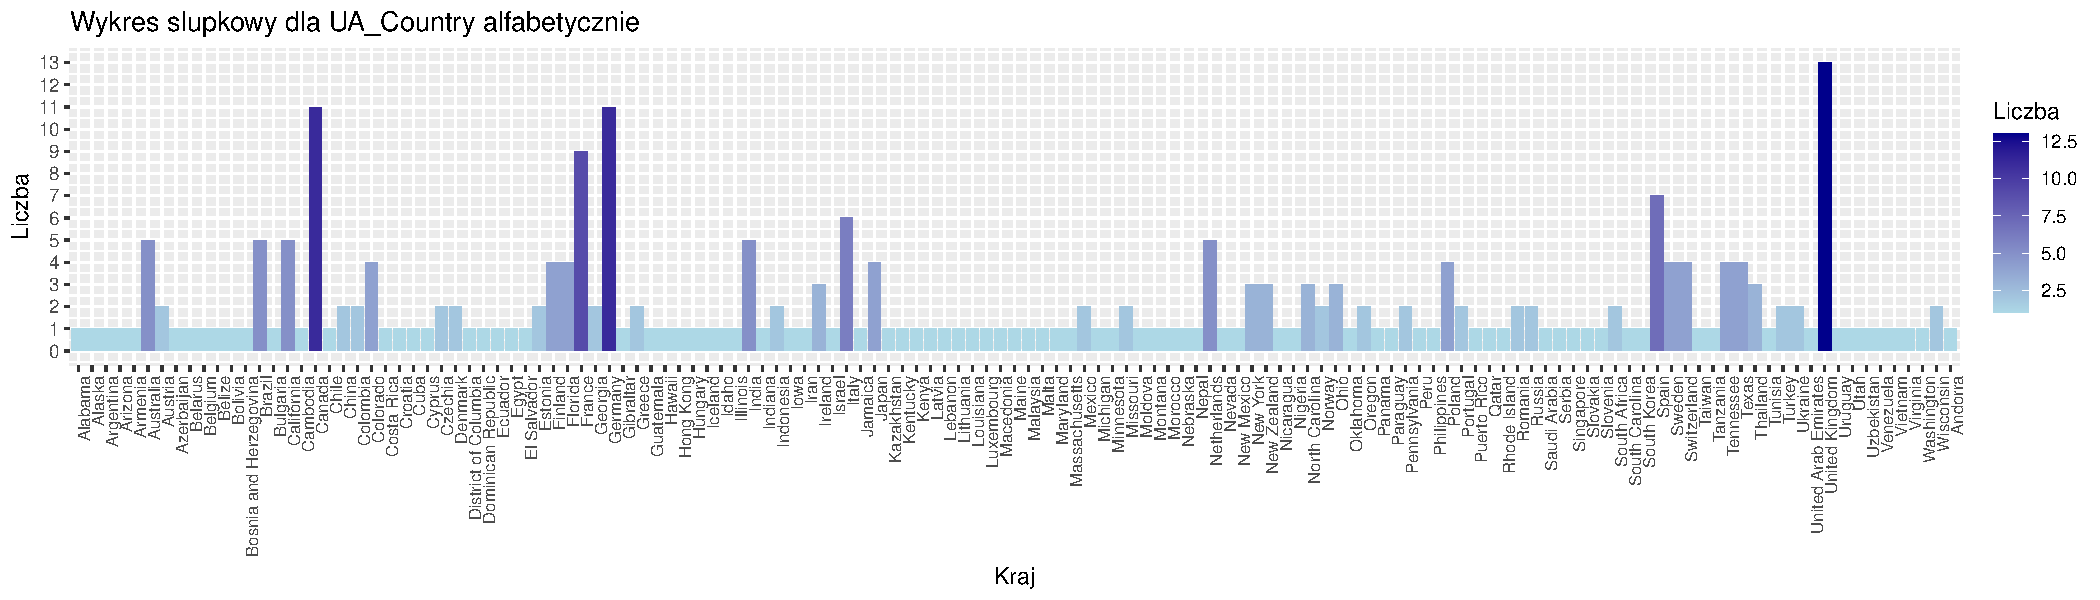
\includegraphics{Sprawozdanie2_files/figure-latex/wykresy_jakosciowe-2} \end{center}

\begin{center}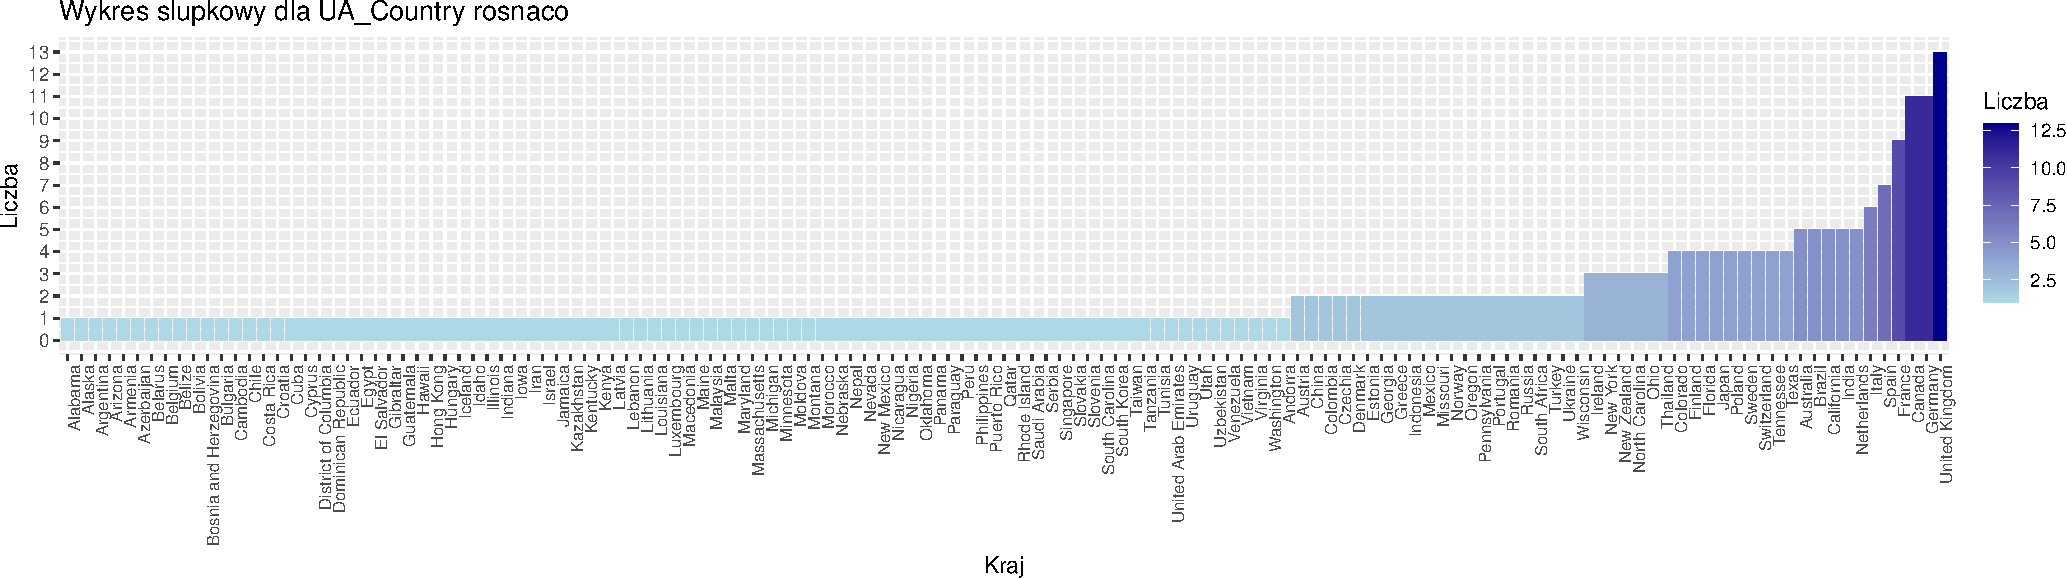
\includegraphics{Sprawozdanie2_files/figure-latex/wykresy_jakosciowe-3} \end{center}

\begin{center}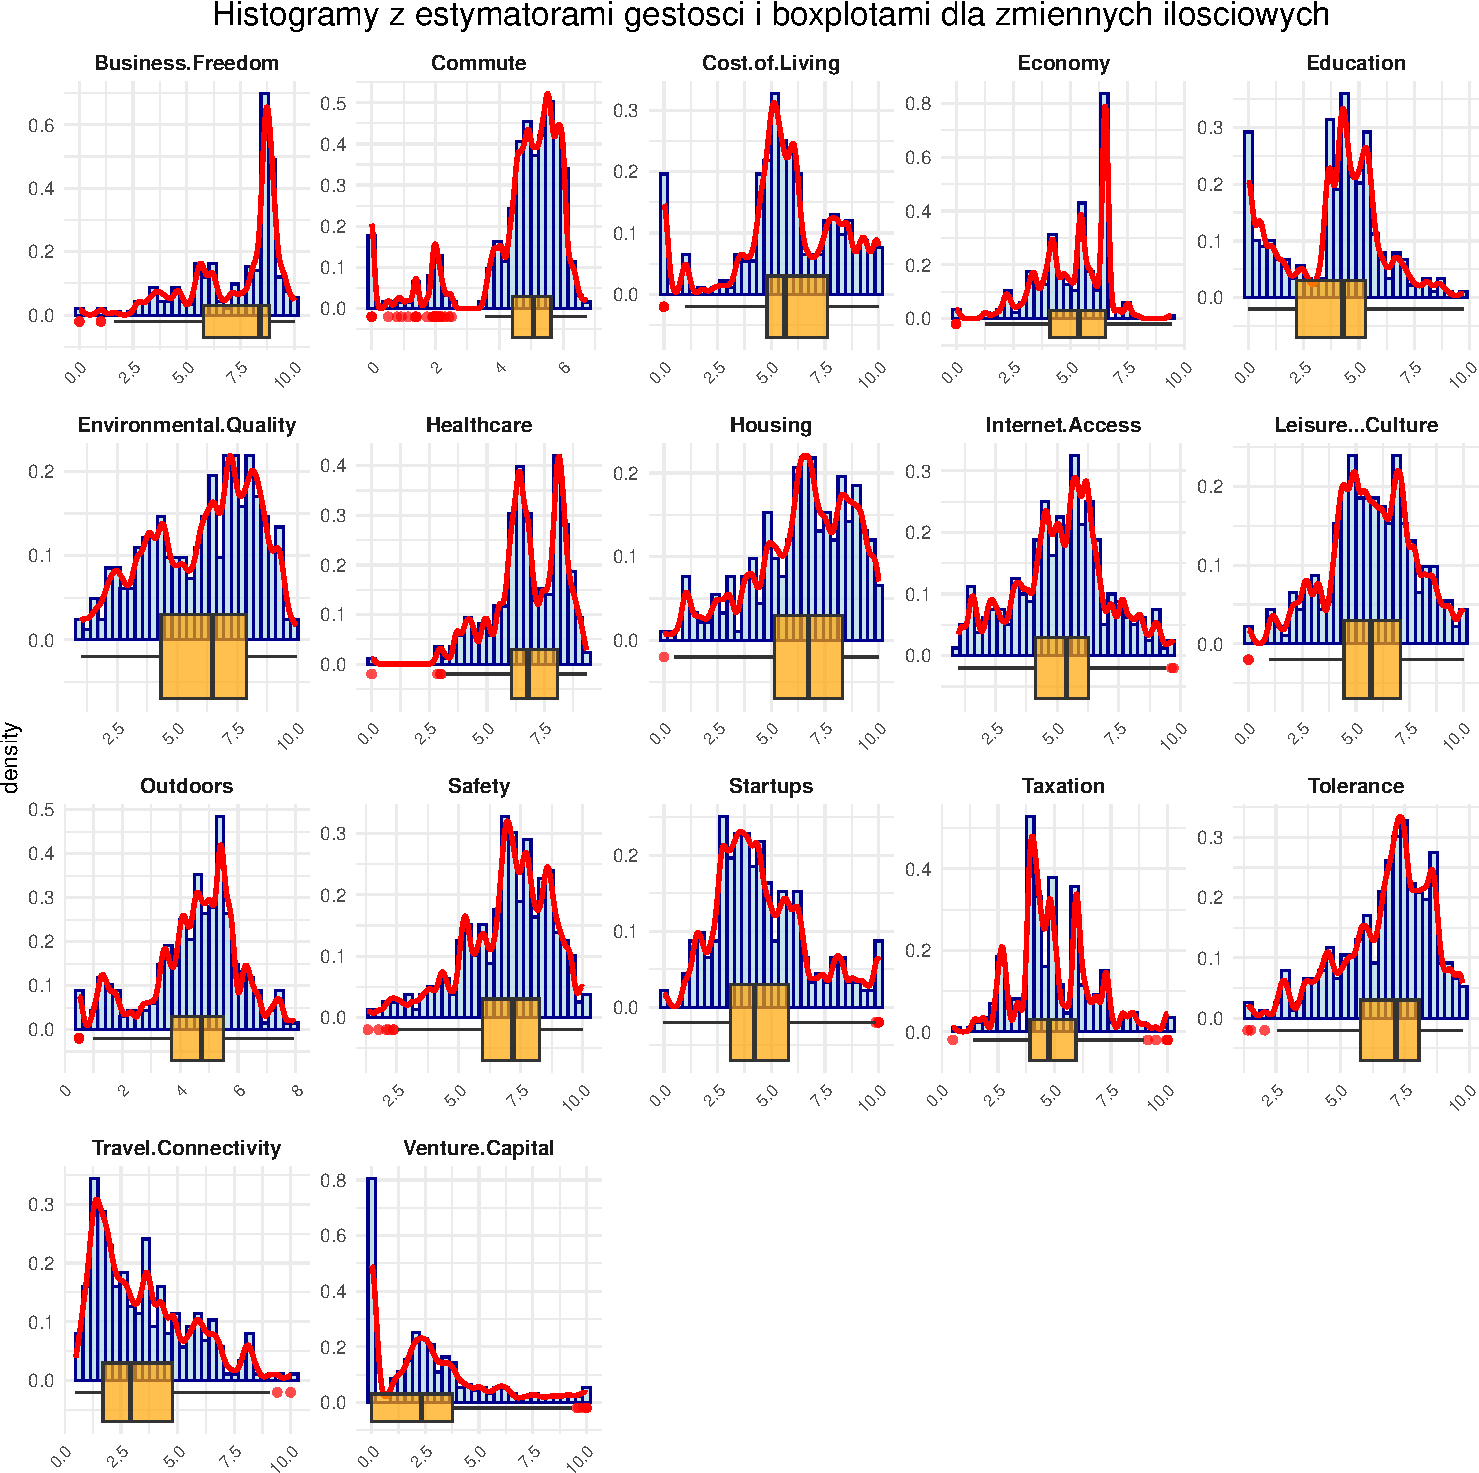
\includegraphics{Sprawozdanie2_files/figure-latex/histogramy_ilosciowe1-1} \end{center}

\begin{center}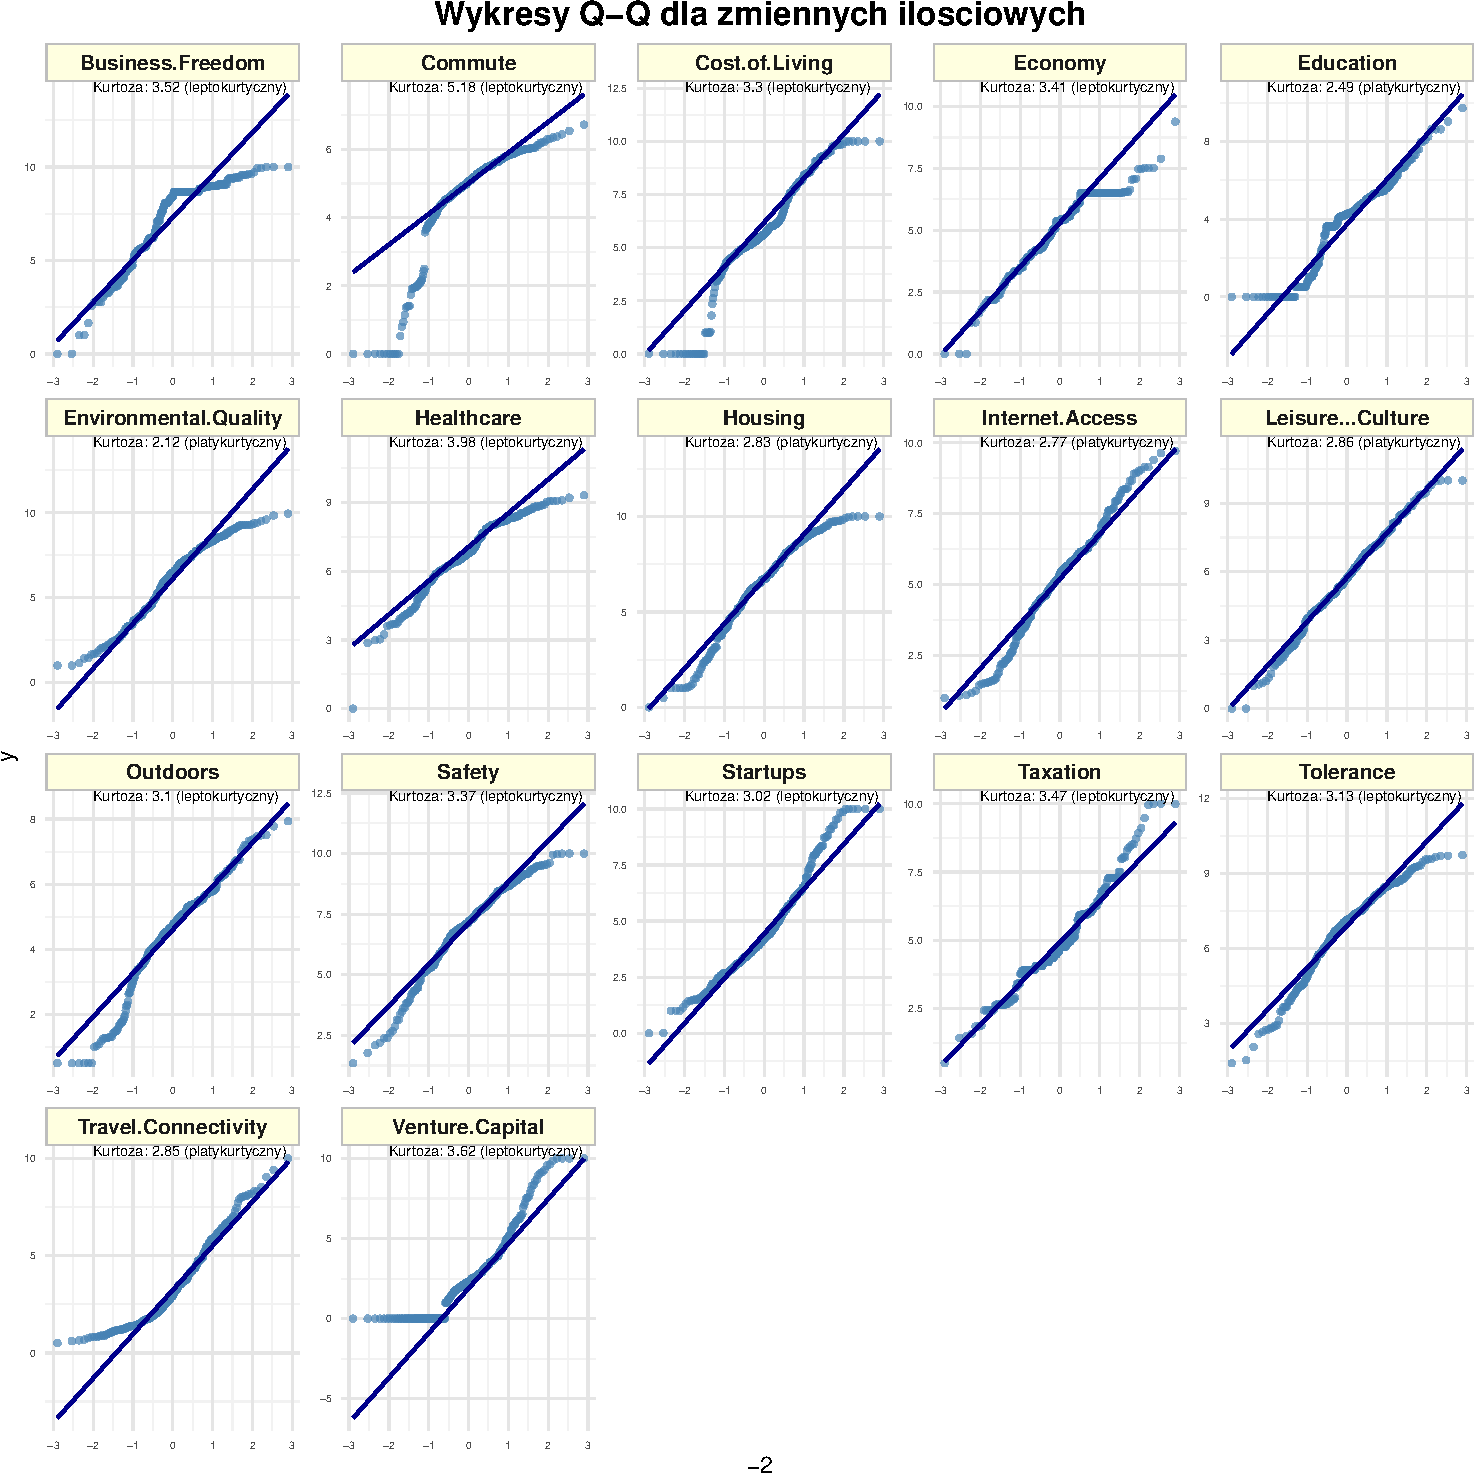
\includegraphics{Sprawozdanie2_files/figure-latex/qq_z_kurtoza-1} \end{center}

\begin{center}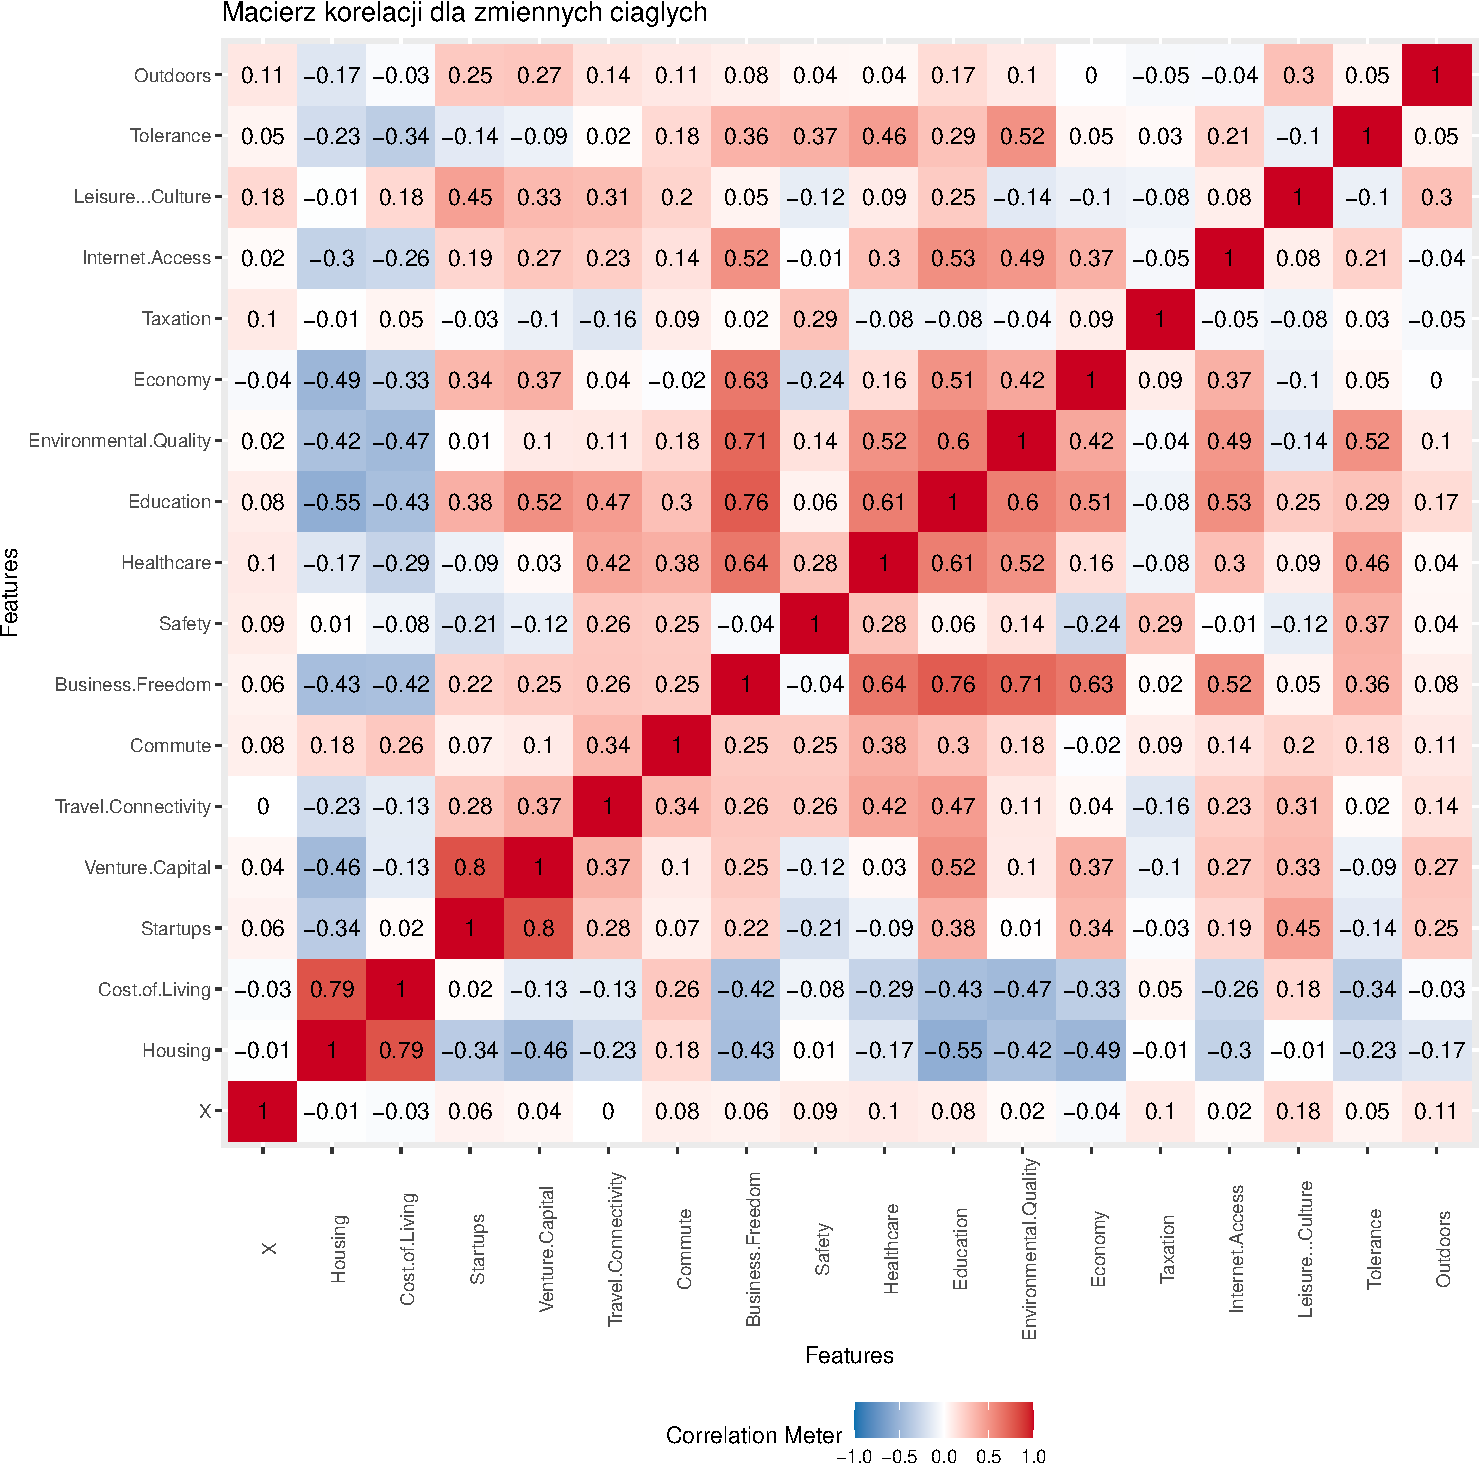
\includegraphics{Sprawozdanie2_files/figure-latex/wykresy_korelacji-1} \end{center}

\begin{center}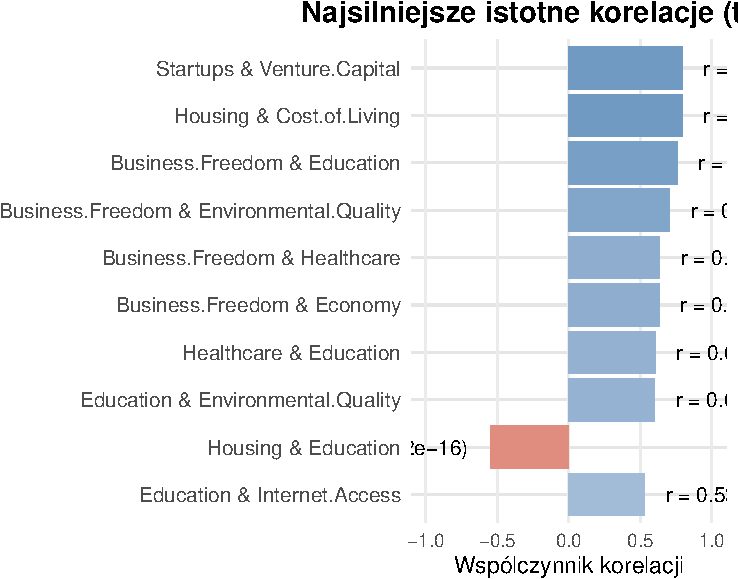
\includegraphics{Sprawozdanie2_files/figure-latex/znaczace_korelacje-1} \end{center}

\begin{longtable}[]{@{}rlllrr@{}}
\toprule\noalign{}
X & UA\_Name & UA\_Country & UA\_Continent & Housing & Cost.of.Living \\
\midrule\noalign{}
\endhead
\bottomrule\noalign{}
\endlastfoot
0 & Aarhus & Denmark & Europe & 6.132 & 4.015 \\
1 & Adelaide & Australia & Oceania & 6.310 & 4.692 \\
2 & Albuquerque & New Mexico & North America & 7.262 & 6.059 \\
3 & Almaty & Kazakhstan & Asia & 9.282 & 9.333 \\
4 & Amsterdam & Netherlands & Europe & 3.053 & 3.824 \\
5 & Anchorage & Alaska & North America & 5.434 & 3.141 \\
\end{longtable}

\begin{longtable}[]{@{}rrrrrr@{}}
\toprule\noalign{}
X & Startups & Venture.Capital & Travel.Connectivity & Commute &
Business.Freedom \\
\midrule\noalign{}
\endhead
\bottomrule\noalign{}
\endlastfoot
0 & 2.827 & 2.512 & 3.536 & 6.312 & 9.940 \\
1 & 3.136 & 2.640 & 1.777 & 5.336 & 9.400 \\
2 & 3.772 & 1.493 & 1.456 & 5.056 & 8.671 \\
3 & 2.458 & 0.000 & 4.592 & 5.871 & 5.568 \\
4 & 7.972 & 6.107 & 8.325 & 6.118 & 8.837 \\
5 & 2.795 & 0.000 & 1.738 & 4.715 & 8.671 \\
\end{longtable}

\begin{longtable}[]{@{}rrrrrr@{}}
\toprule\noalign{}
X & Safety & Healthcare & Education & Environmental.Quality & Economy \\
\midrule\noalign{}
\endhead
\bottomrule\noalign{}
\endlastfoot
0 & 9.617 & 8.704 & 5.367 & 7.633 & 4.887 \\
1 & 7.926 & 7.937 & 5.142 & 8.331 & 6.070 \\
2 & 1.343 & 6.430 & 4.152 & 7.319 & 6.514 \\
3 & 7.309 & 4.546 & 2.283 & 3.857 & 5.269 \\
4 & 8.504 & 7.907 & 6.180 & 7.597 & 5.053 \\
5 & 3.470 & 6.060 & 3.624 & 9.272 & 6.514 \\
\end{longtable}

\begin{longtable}[]{@{}rrrrrr@{}}
\toprule\noalign{}
X & Taxation & Internet.Access & Leisure\ldots Culture & Tolerance &
Outdoors \\
\midrule\noalign{}
\endhead
\bottomrule\noalign{}
\endlastfoot
0 & 5.068 & 8.373 & 3.187 & 9.739 & 4.130 \\
1 & 4.588 & 4.341 & 4.328 & 7.822 & 5.531 \\
2 & 4.346 & 5.396 & 4.890 & 7.028 & 3.515 \\
3 & 8.522 & 2.886 & 2.937 & 6.540 & 5.500 \\
4 & 4.955 & 4.523 & 8.874 & 8.368 & 5.307 \\
5 & 4.772 & 4.964 & 3.266 & 7.093 & 5.358 \\
\end{longtable}

\begin{longtable}[]{@{}lr@{}}
\toprule\noalign{}
& Wariancja \\
\midrule\noalign{}
\endhead
\bottomrule\noalign{}
\endlastfoot
Housing & 5.265 \\
Cost.of.Living & 5.988 \\
Startups & 4.635 \\
Venture.Capital & 6.520 \\
Travel.Connectivity & 4.375 \\
Commute & 2.320 \\
Business.Freedom & 4.450 \\
Safety & 3.051 \\
Healthcare & 2.196 \\
Education & 4.897 \\
Environmental.Quality & 4.840 \\
Economy & 2.302 \\
Taxation & 2.855 \\
Internet.Access & 3.505 \\
Leisure\ldots Culture & 4.027 \\
Tolerance & 2.974 \\
Outdoors & 2.534 \\
\end{longtable}

\begin{center}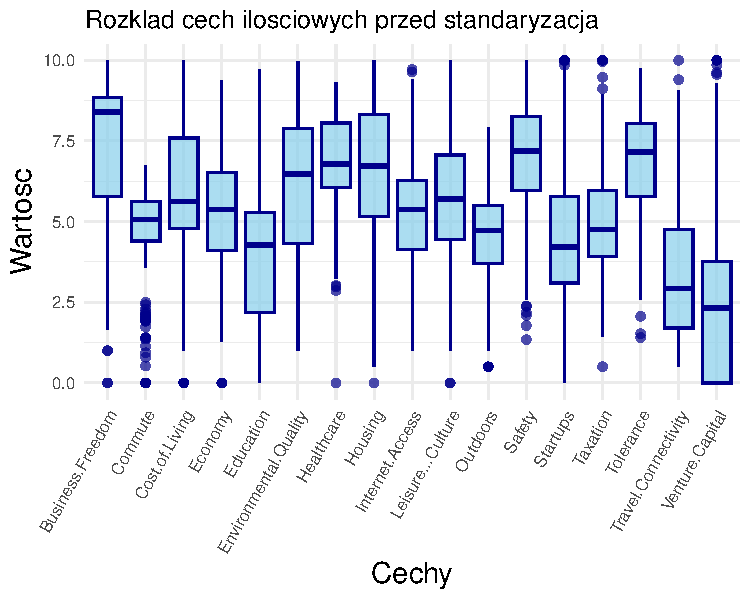
\includegraphics{Sprawozdanie2_files/figure-latex/wykresy_rozkładów_standaryzacja_boxplot-1} \end{center}

\begin{center}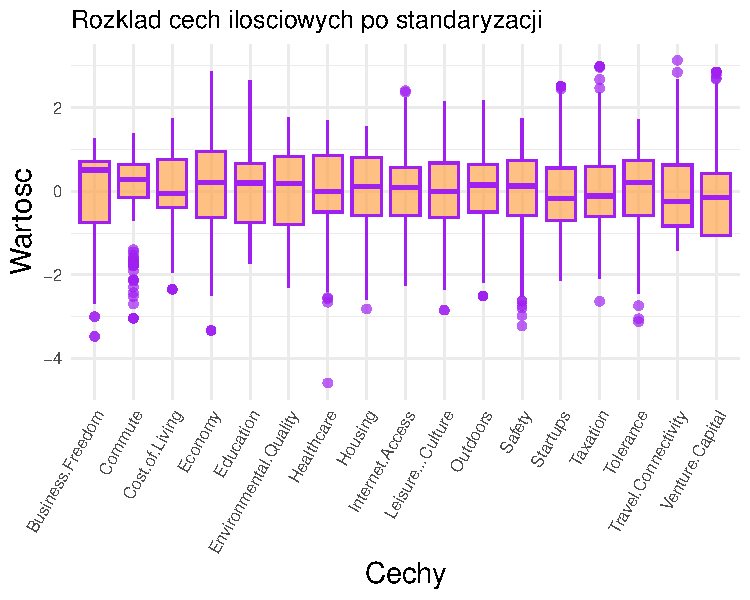
\includegraphics{Sprawozdanie2_files/figure-latex/wykresy_rozkładów_standaryzacja_boxplot-2} \end{center}

\subsection{b) Wyznaczenie składowych
głównych}\label{b-wyznaczenie-skux142adowych-gux142uxf3wnych}

\begin{longtable}[]{@{}lrrr@{}}
\caption{Podsumowanie analizy PCA}\tabularnewline
\toprule\noalign{}
Składowa & Odchylenie\_standardowe & Procent\_wariancji &
Kumulatywna\_wariancja \\
\midrule\noalign{}
\endfirsthead
\toprule\noalign{}
Składowa & Odchylenie\_standardowe & Procent\_wariancji &
Kumulatywna\_wariancja \\
\midrule\noalign{}
\endhead
\bottomrule\noalign{}
\endlastfoot
PC1 & 2.251 & 29.80 & 29.80 \\
PC2 & 1.606 & 15.16 & 44.96 \\
PC3 & 1.443 & 12.25 & 57.21 \\
PC4 & 1.140 & 7.65 & 64.86 \\
PC5 & 1.095 & 7.05 & 71.90 \\
PC6 & 0.980 & 5.65 & 77.55 \\
PC7 & 0.831 & 4.06 & 81.62 \\
PC8 & 0.815 & 3.90 & 85.52 \\
PC9 & 0.764 & 3.43 & 88.95 \\
PC10 & 0.651 & 2.50 & 91.45 \\
PC11 & 0.569 & 1.90 & 93.35 \\
PC12 & 0.539 & 1.71 & 95.06 \\
PC13 & 0.524 & 1.62 & 96.68 \\
PC14 & 0.434 & 1.11 & 97.79 \\
PC15 & 0.393 & 0.91 & 98.69 \\
PC16 & 0.352 & 0.73 & 99.42 \\
PC17 & 0.313 & 0.58 & 100.00 \\
\end{longtable}

\subsection{c) Zmienność odpowiadająca poszczególnym
składowym}\label{c-zmiennoux15bux107-odpowiadajux105ca-poszczeguxf3lnym-skux142adowym}

\begin{center}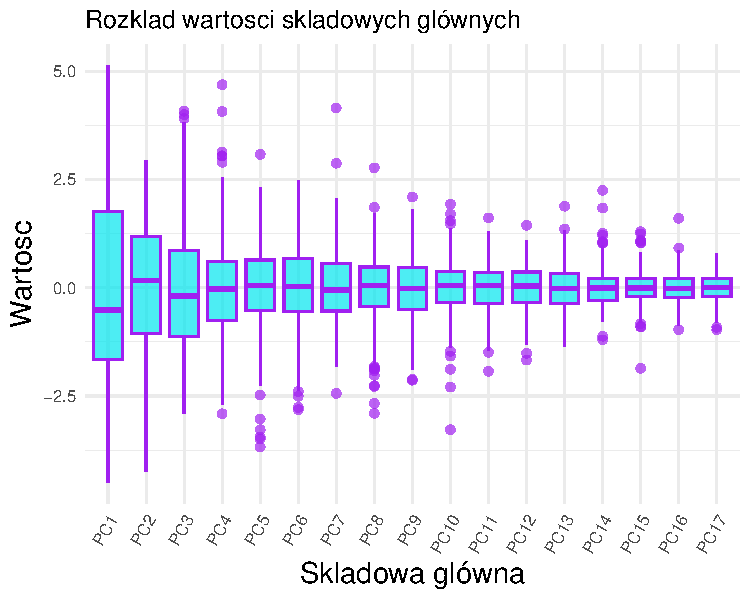
\includegraphics{Sprawozdanie2_files/figure-latex/rozklad_wartosci_wykres_boxplot-1} \end{center}

\begin{longtable}[t]{lrrr}
\caption{\label{tab:ladunki}Wektory ładunków dla PC1, PC2 i PC3}\\
\toprule
\cellcolor[HTML]{f2f2f2}{\textbf{}} & \cellcolor[HTML]{f2f2f2}{\textbf{PC1}} & \cellcolor[HTML]{f2f2f2}{\textbf{PC2}} & \cellcolor[HTML]{f2f2f2}{\textbf{PC3}}\\
\midrule
Housing & 0.3078251 & 0.0533534 & -0.3135465\\
Cost.of.Living & 0.2596091 & -0.1757815 & -0.3305352\\
Startups & -0.1802385 & -0.4834415 & 0.0061000\\
Venture.Capital & -0.2365974 & -0.4274509 & 0.0148768\\
Travel.Connectivity & -0.2094543 & -0.1353067 & -0.3397760\\
\addlinespace
Commute & -0.1142045 & 0.0259310 & -0.5057359\\
Business.Freedom & -0.3772809 & 0.0982196 & 0.0241046\\
Safety & -0.0389355 & 0.2871039 & -0.3330100\\
Healthcare & -0.2803590 & 0.2419482 & -0.2810248\\
Education & -0.4025620 & -0.0490795 & -0.0738645\\
\addlinespace
Environmental.Quality & -0.3262220 & 0.2525355 & 0.0535717\\
Economy & -0.2731752 & -0.0740033 & 0.3086705\\
Taxation & 0.0262992 & 0.1074151 & -0.0201849\\
Internet.Access & -0.2761922 & 0.0227056 & 0.0284416\\
Leisure...Culture & -0.0744466 & -0.3647324 & -0.3050545\\
\addlinespace
Tolerance & -0.1897496 & 0.3550911 & -0.1027251\\
Outdoors & -0.0915866 & -0.1933825 & -0.1485868\\
\bottomrule
\end{longtable}

\begin{center}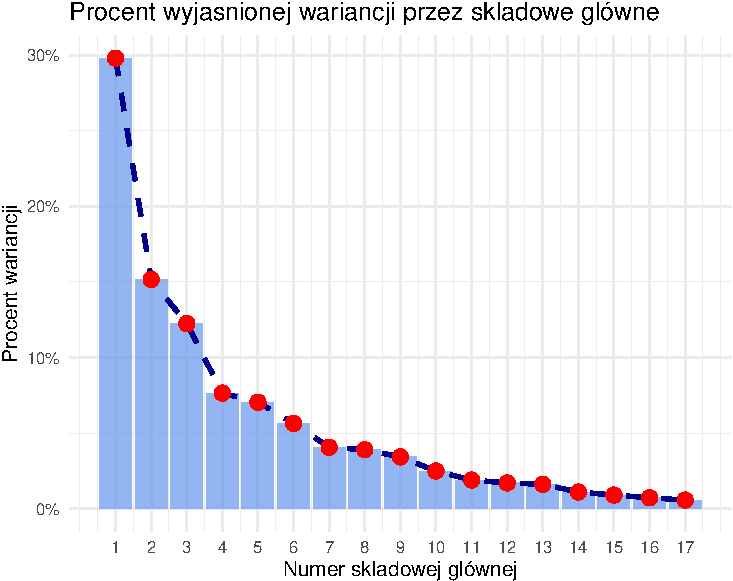
\includegraphics{Sprawozdanie2_files/figure-latex/Zmiennosc_skladowych_w_PCA-1} \end{center}

\begin{center}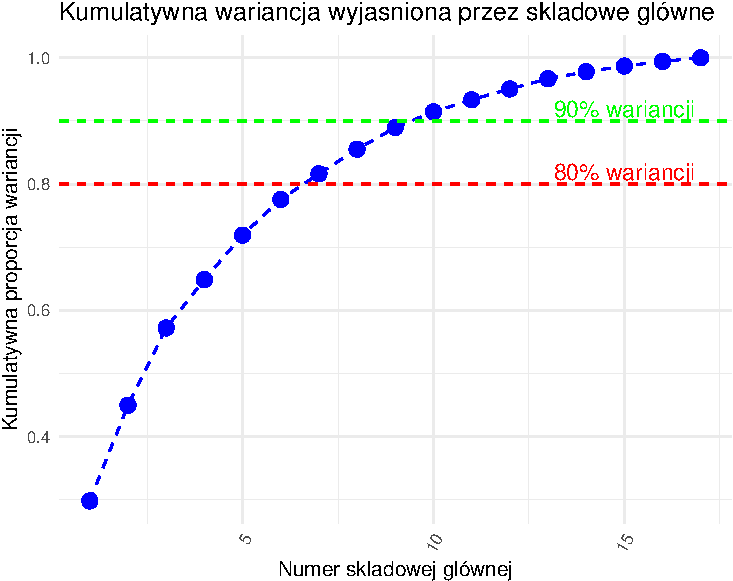
\includegraphics{Sprawozdanie2_files/figure-latex/Zmiennosc_skladowych_w_PCA-2} \end{center}

Liczba składowych głównych wyjaśniających \textbf{80\%} wariancji:
\textbf{7}\\
Liczba składowych głównych wyjaśniających \textbf{90\%} wariancji:
\textbf{10}

\subsection{d) Wizualizacja danych
wielowymiarowych}\label{d-wizualizacja-danych-wielowymiarowych}

\subsection{e) Korelacja zmiennych}\label{e-korelacja-zmiennych}

\subsection{d) Wizualizacja danych
wielowymiarowych}\label{d-wizualizacja-danych-wielowymiarowych-1}

\subsection{e) Korelacja zmiennych}\label{e-korelacja-zmiennych-1}

\subsection{f) Końcowe wnioski}\label{f-koux144cowe-wnioski}

\subsection{f) Końcowe wnioski}\label{f-koux144cowe-wnioski-1}

\section{ZADANIE 3 (Skalowaniewielowymiarowe (Multidimensional Scaling
(MDS)))}\label{zadanie-3-skalowaniewielowymiarowe-multidimensional-scaling-mds}

\subsection{a) Dane: titanic\_train (R-pakiet
titanic)}\label{a-dane-titanic_train-r-pakiet-titanic}

Zbiór danych zawiera wybrane charakterystyki opisujące pasażerów
Titanica (w tym m.in. takie zmienne jak: wiek, płeć, miejsce rozpoczęcia
podróży czy klasa pasażerska) wraz z informacją czy dana osoba przeżyła
katastrofę (zmienna Survived).

\subsection{b) Przygotowanie danych}\label{b-przygotowanie-danych}

Wczytane dane, niepotrzebne kolumny zostały usunięte, oraz typy
poszczególnych cech zostały zaaktualizowane na odpowiednie czyt.
ordered,numeric

\subsection{c) Redukcja wymiaru na bazie
MDS}\label{c-redukcja-wymiaru-na-bazie-mds}

Redukuję wymiar danych korzystając z \textbf{metody metrycznej (Funkcja
cmdscale)}

Kolejno tworzymy diagram Shepherda

\begin{center}\includegraphics{Sprawozdanie2_files/figure-latex/diagram shepherda-1} \end{center}

Widać, że odległości w nowej przestrzeni danych zmieniły się, nadal mają
podobny charakter, największe skupisko danych znajduje się przy lini x =
y (w gdyby odległości zostały zachwoane, czyli w idealnym scenariuszu,
to nasze nowe odległości przechodziły by właśnie przez tą linię).

Pomimo, że duża liczba punktów odbiega od lini x = y , to jednak różnica
między ich nową odległością a starą nie są duże (nie mamy znaczących
rozrzutów na osi OY), więc możemy uznać skalowanie za dość dobre, chyba
,że chcemy przeprowadzać bardzo dokładną analizę

\subsection{d) Wizualizacja danych}\label{d-wizualizacja-danych}

\begin{center}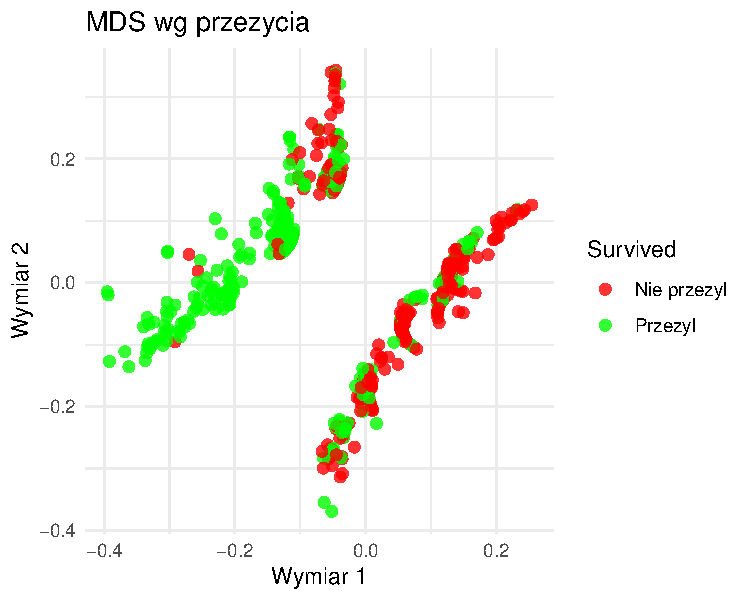
\includegraphics{Sprawozdanie2_files/figure-latex/rozrzut 2D-1} \end{center}

\end{document}
